\documentclass[11pt,a4paper]{article}
\usepackage[utf8]{inputenc}
\usepackage{amsmath}
\usepackage{amsfonts}
\usepackage{amssymb}
\usepackage[left=2cm,right=2cm,top=2cm,bottom=2cm]{geometry}


\usepackage{slashed}
\usepackage{hyperref}
\usepackage{graphicx}
\usepackage{caption}
\usepackage{float}
\usepackage{subcaption}

\usepackage{minted}
\usepackage[dvipsnames]{xcolor}


\renewcommand{\theequation}{\arabic{section}.\arabic{equation}}



\usepackage{ifthen}
\usepackage[dvipsnames]{xcolor}
\usepackage{tikz}


%Define color environments:

\newenvironment{DK}[1]{{\color{gray}Commend from D: #1}}

\newenvironment{DKnew}[1]{{\color{blue}NEW from D: #1}}

\newenvironment{DKres}[1]{{\color{BrickRed}RESTRUCTURED from D: #1}}




\newcommand{\dint}{  \displaystyle \int }
%%%%%%%%%%%%%%%%%%%%%%%%%%%%%%%%%%%%%%%%%%
\newcommand{\ie}{{\em i.e.} }
\newcommand{\eg}{{\em e.g.} }
\newcommand{\GeV}{{\rm GeV}}
\newcommand{\TeV}{{\rm TeV}}
\newcommand{\MeV}{{\rm MeV}}
\newcommand{\keV}{{\rm keV}}

\newcommand{\rhs}{RHS }
\newcommand{\lhs}{LHS }


\newcommand{\geff}{ g_{\rm eff} }
\newcommand{\heff}{ h_{\rm eff} }
 
\newcommand{\Ham}{ \mathcal{H} }
 
\newcommand{\thetamax}{ \theta_{\rm max}{} }

 
\newcommand{\thetai}{ \theta_{\rm ini}{} }

\newcommand{\fa}{ f_{\alpha}{} }
 
\newcommand{\ti}{ t_{\rm ini}{} }
 
\newcommand{\Ri}{ R_{\rm ini}{} }


\newcommand{\tosc}{ t_{\rm osc}{} }

\newcommand{\Omegai}{ \Omega_{\rm ini} }
 
\newcommand{\ma}{ m_\alpha{} }

\newcommand{\Lint}{ \mathcal{L}_{\rm int} }


\newcommand{\vev}[1]{\langle #1 \rangle}
\newcommand{\Bvev}[1]{\Bigg\langle #1 \Bigg\rangle}
\newcommand{\bvev}[1]{\Big\langle #1 \Big\rangle}




\newcommand{\lrb}[1]{\left( #1 \right)}
\newcommand{\lrsb}[1]{\left[ #1 \right]}
\newcommand{\lrBigb}[1]{\Big( #1 \Big)}
\newcommand{\lrBigsb}[1]{\Big[ #1 \Big]}
\newcommand{\lrBiggb}[1]{\Bigg( #1 \Bigg)}
\newcommand{\lrBiggsb}[1]{\Bigg[ #1 \Bigg]}

\newcommand{\lrBigcb}[1]{\Big\{ #1 \Big\}}
\newcommand{\lrBiggcb}[1]{\Bigg\{ #1 \Bigg\}}
%%%%%%%%%%%%%%%%%%%%%%%%%%%%%%%%%%%%%%%%%

%%%%%%%%%%%%%%%%%%%%%%%%%%%%%%%%%%%%%%%%%%%%%%%%%%%--Begin_refs--%%%%%%%%%%%%%%%%%%%%%%%%%%%%%%%%%%%%%%%%%%%%%%%%%%%%%%%%%%%%%%%%%%%%%%
\newcounter{NumArgs}

%Define reference to an arbitrary number of equations (\eqs{label_1,label_2....,label_n} will show eqs. ref_1, ref_2, ..., and ref_n)
\newcommand{\eqs}[1]{\setcounter{NumArgs}{0}\foreach\i in{#1}{\stepcounter{NumArgs}}%
\ifthenelse{\equal{\theNumArgs}{1}}{eq.~(\ref{#1})}%
{\ifthenelse{\equal{\theNumArgs}{2}}%
{eqs.~\foreach\i[count=\q]in{#1}{\ifthenelse{\equal{\q}{\theNumArgs}}{and (\ref{\i})}{(\ref{\i})~}}}%
{eqs.~\foreach\i[count=\q]in{#1}{\ifthenelse{\equal{\q}{\theNumArgs}}{and (\ref{\i})}{(\ref{\i}),~}}}}}


%Define reference to an arbitrary number of equations (\Eqs{label_1,label_2....,label_n} will show Eqs. ref_1, ref_2, ..., and ref_n)
\newcommand{\Eqs}[1]{\setcounter{NumArgs}{0}\foreach\i in{#1}{\stepcounter{NumArgs}}%
\ifthenelse{\equal{\theNumArgs}{1}}{Eq.~(\ref{#1})}%
{\ifthenelse{\equal{\theNumArgs}{2}}%
{Eqs.~\foreach\i[count=\q]in{#1}{\ifthenelse{\equal{\q}{\theNumArgs}}{and (\ref{\i})}{(\ref{\i})~}}}%
{Eqs.~\foreach\i[count=\q]in{#1}{\ifthenelse{\equal{\q}{\theNumArgs}}{and (\ref{\i})}{(\ref{\i}),~}}}}}


%Define reference to an arbitrary number of labels (\REF{label_1,label_2....,label_n} will show ref_1, ref_2, ..., and ref_n)
\newcommand{\refs}[1]{\setcounter{NumArgs}{0}\foreach\i in{#1}{\stepcounter{NumArgs}}%
\ifthenelse{\equal{\theNumArgs}{1}}{(\ref{#1})}%
{\ifthenelse{\equal{\theNumArgs}{2}}%
{\foreach\i[count=\q]in{#1}{\ifthenelse{\equal{\q}{\theNumArgs}}{and (\ref{\i})}{(\ref{\i})~}}}%
{\foreach\i[count=\q]in{#1}{\ifthenelse{\equal{\q}{\theNumArgs}}{and (\ref{\i})}{(\ref{\i}),~}}}}}



%Define reference to an arbitrary number of figs (\Figs{label_1,label_2....,label_n} will show ref_1, ref_2, ..., and ref_n)
\newcommand{\Figs}[1]{\setcounter{NumArgs}{0}\foreach\i in{#1}{\stepcounter{NumArgs}}%
\ifthenelse{\equal{\theNumArgs}{1}}{Fig.~(\ref{#1})}%
{\ifthenelse{\equal{\theNumArgs}{2}}%
{Figs.~\foreach\i[count=\q]in{#1}{\ifthenelse{\equal{\q}{\theNumArgs}}{and (\ref{\i})}{(\ref{\i})~}}}%
{Figs.~\foreach\i[count=\q]in{#1}{\ifthenelse{\equal{\q}{\theNumArgs}}{and (\ref{\i})}{(\ref{\i}),~}}}}}




%Define reference to an arbitrary number of "general reference" (\Gen{message}{label_1,label_2....,label_n} will show message.(ref_1), (ref_2), ..., and (ref_n)
\newcommand{\Gen}[2]{\setcounter{NumArgs}{0}\foreach\i in{#2}{\stepcounter{NumArgs}}%
	\ifthenelse{\equal{\theNumArgs}{1}}{#1.~(\ref{#2})}%
	{\ifthenelse{\equal{\theNumArgs}{2}}%
		{#1.~\foreach\i[count=\q]in{#2}{\ifthenelse{\equal{\q}{\theNumArgs}}{and (\ref{\i})}{(\ref{\i})~}}}%
		{#1.~\foreach\i[count=\q]in{#2}{\ifthenelse{\equal{\q}{\theNumArgs}}{and (\ref{\i})}{(\ref{\i}),~}}}}}


%%%%%%%%%%%%%%%%%%%%%%%%%%%%%%%%%%%%%%%%%%%%%%%%%%%--End_refs--%%%%%%%%%%%%%%%%%%%%%%%%%%%%%%%%%%%%%%%%%%%%%%%%%%%%%%%%%%%%%%%%%%%%%%



%%%%%%%-----------------------Rules-----------------------%%%%%%%
% 1. Put any new macros in macros.tex.

% 2. Section should start with:
	%\section{This is a section}\label{sec:Intro}
	%\setcounter{equation}{0}

% 3. labels for Figs should start with fig:, for equations should start with eq:, for sections with sec:, etc.
%%%%%%%--------------------------------------------------%%%%%%%




\author{Karamitros Dimitrios}
\title{{\tt MiMeS}: Misalignment Mechanism Solver}
\begin{document}

\maketitle

\begin{abstract}
	We introduce a \CPP header-only library that solves the Axion equation of motion, \mimes.  
	\mimes makes no assumptions regarding the cosmology and the thermal mass of the axion, which allows the user 
	to consider various cosmological scenarios and axion-like models.
	Moreover, although written entirely in \CPP, \mimes comes with a convenient \PY interface, which does not require the
	user to write any code in \CPP.
\end{abstract}


\section{Introduction}\label{sec:intro}
\setcounter{equation}{0}

About the axion...

\section{Axion relic abundance}\label{sec:abundance}
\setcounter{equation}{0}
%
Although there are several works in the literature that (such as~\cite{Chang:1998ys}) that can also provide a useful insight on the solution of the axion equation of motion (EOM), it would be useful to derive and define the quantities we need in this section, in order to understand how \mimes works in detail.

\paragraph{The EOM} The axion field is written as 
%
\begin{equation}
	a  \equiv \fa \ \theta,
	\label{eq:fa_def}
\end{equation}
%
with $\fa$ the scale of the axion that determines the the scale at which the PQ symmetry breaks. 

The EOM in terms of $\theta$ is 
%
\begin{equation}
	\lrb{\dfrac{d^2}{d t^2} + 3 H(t) \ \dfrac{d}{d t} } \theta(t) + \maT^2(t) \ \sin \theta(t) = 0 \; ,
	\label{eq:eom}
\end{equation}
%
with $H(t)$ the Hubble parameter (determined by the cosmology), and $\maT(t)$  the time (temperature) dependent mass of the axion. 

\paragraph{Initial conditions}
%
\begin{figure}[h!]
	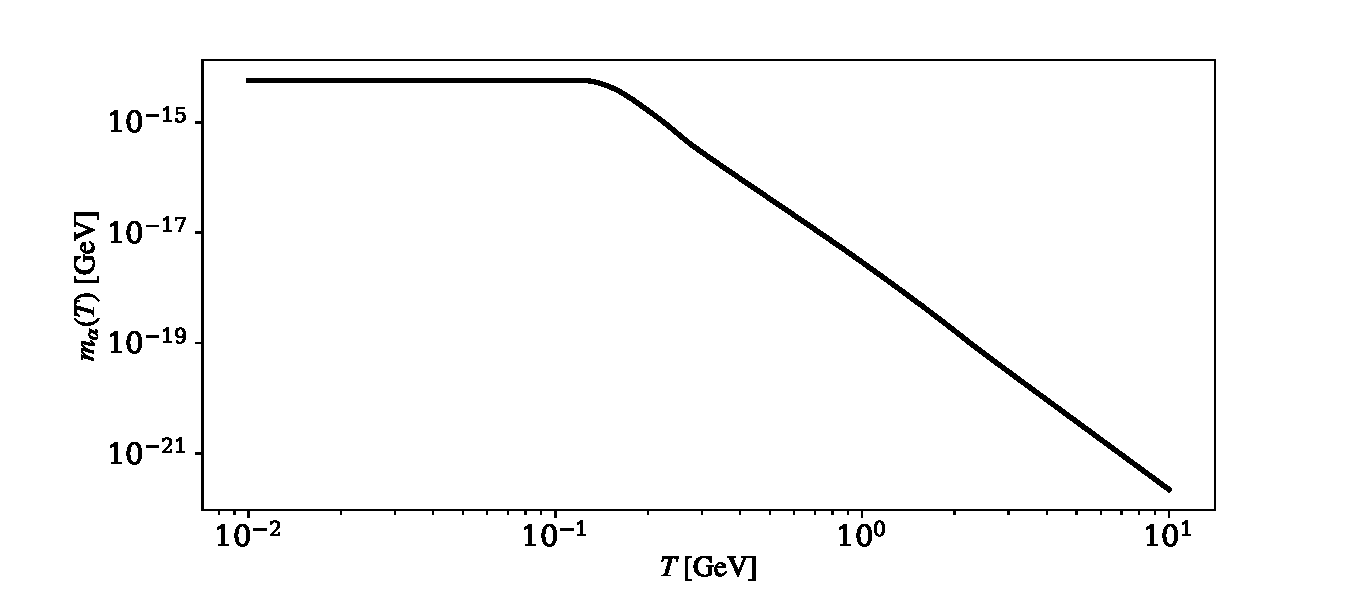
\includegraphics[width=1\textwidth]{figs/axion_mass.pdf}
	\caption{The mass of the axion as a function of the temperature for $\fa=10^{12}~\GeV$, using the data provided in ref.~\cite{Borsanyi:2016ksw}.}
	\label{fig:axion_mass}
\end{figure}
%
Assuming that the PQ symmetry breaks before inflation, the initial conditions (\ie at some $t=0$, after inflation) for the EOM is random. However, we note that $\maT \to 0$ (see \Figs{fig:axion_mass}) -- \ie $\maT \ll H$ -- at very early times. Therefore, after inflation, the EOM becomes
%
\begin{equation}
	\lrb{\dfrac{d^2}{d t^2} + 3 H(t) \ \dfrac{d}{d t}  } \theta(t) = 0 \; ,
	\label{eq:massless_eom}
\end{equation}
%
which is solved by $\theta = \thetai + C \dint_{0}^t d t \ \lrb{ \dfrac{R_{0}}{R(t)} }^3$. That is, as the Universe expands, $\theta \approx \thetai$. Since we would like to calculate the relic abundance of axions, we can integrate \eqs{eq:eom} from a time after inflation (call it $t = \ti$) such that $ \dot \theta |_{t=\ti} = 0$ and  $\theta|_{t=\ti} \approx \thetai$.   



\subsection{The WKB approximation}
%
In order to solve analytically \eqs{eq:eom}, we assume $\theta \ll 1$, which results in the linearised EOM
%
\begin{equation}
	\lrb{\dfrac{d^2}{d t^2} + 3 H(t) \ \dfrac{d}{d t} + \maT^2(t) } \theta(t) = 0 \; .
	\label{eq:linear_eom}
\end{equation}

Using a trial solution $\psi = \exp\lrsb{ i \dint d t \ \lrBigb{u(t) +3/2 \ i \ H(t)} }$, and defining $\Omega^2 = \maT^2 - \dfrac{9}{4} H^2 -  \dfrac{3}{2} \dot H $ we can transform the \eqs{eq:linear_eom} to 
%
\begin{equation}
	u^2 = \Omega^2 + i \ \dot u \; ,
	\label{eq:eom_of_u}
\end{equation}
%
which has a formal solution $u = \pm \sqrt{\Omega^2 + i \dot u}$. Assuming that $\dot u \ll \Omega^2$ and $\dot \Omega \ll \Omega^2$, we can approximate $u$ as
%
\begin{equation}
	u \approx \pm \Omega + \dfrac{i}{2} \dfrac{d \log \Omega}{d t} \;,
	\label{eq:u_approx}
\end{equation}
%
which results in the general solution of \eqs{eq:linear_eom} 
%
\begin{equation}
	\theta \approx \dfrac{1}{\sqrt{\Omega}} \exp\lrb{-\dfrac{3}{2} \int d t \ H} \lrsb{ A \cos\lrb{ \int d t \ \Omega} +  B \sin\lrb{ \int d t \ \Omega}    } \;. 
	\label{eq:general_solution_eom_approx}
\end{equation}

Applying, then, the initial conditions $ \dot \theta |_{t=\ti} = 0$ and  $\theta|_{t=\ti} \approx \thetai$, we arrive with the solution 
%
\begin{equation}
	\theta(t) \approx \thetai \sqrt{ \dfrac{ \Omegai }{\Omega (t)} } \exp\lrb{-\dfrac{3}{2} \int_{\ti}^t d t^\prime  \ H(t^\prime)} \  \cos\lrb{ \int_{\ti}^t d t^\prime  \ \Omega(t^\prime)}   \;.
	\label{eq:solution_eom_approx} 
\end{equation}


In order to further simplify this approximate result, we note that $\theta$ deviates from $\thetai$ only after the mass becomes comparable to the expansion rate of the Universe, \ie after $\maT|_{t = \tosc} = 3 H|_{t = \tosc}$. This observation allows us to use $\ti = \tosc$.  Moreover, at $t> \tosc$, we can approximate $\Omega \approx \maT$, as $H^2$ and $\dot H$ become much smaller than $\maT^2$ quickly after $t=\tosc$. Finally, the axion angle takes the form
%
\begin{equation}
	\theta(t) \approx \thetai \lrb{\dfrac{3}{4}}^{1/4} \sqrt{ \dfrac{ \maT|_{t=\tosc} }{\maT  (t)} } \exp\lrb{-\dfrac{3}{2} \int_{\tosc}^t d t^\prime  \ H(t^\prime)} \  \cos\lrb{ \int_{\tosc}^t d t^\prime  \ \maT(t^\prime)}   \;.
	\label{eq:solution_eom_approx_final} 
\end{equation}
%
Notice that we have assumed $\thetai \approx \theta|_{t=\tosc}$ as initial condition, which can impact the accuracy of the WKB approximation, as $\dot \theta|_{t=\tosc} \neq 0$.

\paragraph{Axion energy density}
%
The energy density of the axion is 
%
\begin{eqnarray}
	\rho_{a} = \dfrac{1}{2} \fa^2 \lrsb{ \dot{\theta}^2 + \maT^2 \theta^2 } \;.
	\label{eq:rho_a_def} 
\end{eqnarray}
%
For the relic abundance of axions, we need to calculate their energy density at very late times. That is, $\dot \maT = 0$, $\maT \gg H$ and $\dot H \ll H^2$. After some algebra, we obtain the approximate form of the energy density (as a function of the scale factor $R$) 
%
\begin{eqnarray}
	\rho_{a} \approx \dfrac{\ma }{2}  \ \fa^2 \ \thetai^2  \ \maT(R_{\rm osc}) \ \lrb{\dfrac{R_{\rm osc}}{R}}^3 \;,
	\label{eq:rho_a0} 
\end{eqnarray}
%
which shows that the energy density of axions at late times scales as the energy density of matter. Thus, today, the energy density of axions can be found by calculating the entropy injection ($\gamma$) between $\tosc$ and today, \ie
%
\begin{equation}
	R^3 \ s = \gamma \ R_{\rm osc}^3 \ s_{\rm osc} \Rightarrow  \lrb{\dfrac{R_{\rm osc}}{R}}^3 = \gamma^{-1} \dfrac{s}{s_{\rm osc}} \;,
\end{equation}
%
which results in the energy density today
\begin{eqnarray}
	\rho_{a,0} = \gamma^{-1}  \dfrac{s_0}{s_{\rm osc}} \  \dfrac{1 }{2}  \ \fa^2 \ \ma \ \maT_{,{\rm osc}} \ \thetai^2    \;,
	\label{eq:rho_a_approx} 
\end{eqnarray}
with $\ma$ the mass of the axion at $T=0$.
%

\subsection{Notation}\label{sec:notation}
%
%The WKB approximation is very useful in order to understand the evolution of the axion field. However, it fails to explain how the oscillation begins before $\dot \Omega \ll \Omega^2$ is reached. In this section we will try to understand the evolution of the axion as generally as possible. 
%
The EOM~(\ref{eq:eom}) depends on time, which is not very useful variable in a non-standard comsological setting. Therefore, we introduce 
%
\begin{eqnarray}
	u = -\log \dfrac{\Ri}{R} \;,
	\label{eq:natation}
\end{eqnarray}
%
which results in 
%
\begin{eqnarray}
	&\dfrac{d F}{dt} &=  H  \dfrac{d F}{du} 
	\nonumber \\
	&\dfrac{d^2 F}{dt^2} &= H^2 \ \lrb{ \dfrac{d^2 F}{du^2} + \dfrac{1}{2} \dfrac{d \log H^2}{du}  \dfrac{d F}{du} }\;.
	\label{eq:deriv_u}
\end{eqnarray}

The EOM in terms of $u$, then, becomes
%
\begin{equation}
	\dfrac{d^2  \theta}{du^2} + \lrsb{\dfrac{1}{2} \dfrac{d \log H^2}{du} + 3 } \dfrac{d  \theta}{d u} + \ \lrb{\dfrac{\maT}{H}}^2 \ \sin \theta
	=0 \;.
	\label{eq:eom_u}
\end{equation}

Notice that in a radiation dominated Universe
%
$$
\dfrac{d \log H^2}{du} = -\lrb{ \dfrac{d \log g_*}{d \log T} +4 } \delta_h^{-1}\;,
$$
with  $ \delta_h = 1+ \dfrac{1}{3} \dfrac{d \log h_*}{d \log T} $. 
%
In a general cosmological setting, the expansion rate is dominated by an energy density that scales as $\rho \sim R^{-c}$, which results in $\dfrac{d \log H^2}{du}  = -c$. However, close to rapid particle annihilations and decays, the evolution of the energy densities change, and $\dfrac{d \log H^2}{du}$ can only be computed numerically.

\subsection{Beyond the WKB approximation}\label{sec:beyond_WKB}
%
The WKB approximation is very useful, as it helps us understand the evolution of the axion field after it begins to oscillate adiabatically. However, it fails to capture the dynamics the adiabatic conditions are met, result in inaccurate axion relic abundance result. In this section, we examine the deviation of $\thetaosc$ from the initial value of $\theta$, as well how to treat cases where the EOM cannot be linearized.

\subsubsection{Behaviour close to the initial condition}\label{sec:close_to_ini}
%
The accuracy of the approximate evolution of the axion angle given in \eqs{eq:solution_eom_approx_final} depends on the deviation between $\thetai$ and $\thetaosc$. In order to examine their deviation, we expand \eqs{eq:eom} at a time $t =\ti + \delta t$ with $\delta t \to 0$. That is, we use the following approximations 
%
\begin{equation*}
	\ddot{\theta} \approx \dfrac{\dot \theta (\ti+ \delta t)  - \dot \theta (\ti)}{ \delta  t } =  \dfrac{\dot \theta (\ti + \delta t)  }{\delta  t } \;,
	\qquad
	\dot \theta(\ti + \delta t) = \dfrac{\theta(\ti + \delta t) - \thetai}{\delta t} \;.
\end{equation*} 
%
and, solve the EOM~\ref{eq:eom} for $\theta(\ti + \delta t)$. This results in
%
\begin{equation}
	\theta(\ti + \delta t)  \approx  \thetai -\dfrac{\delta t^2}{1+3 \ H \ \delta t} \  \maT^2  \sin \theta(\ti + \delta t)  
	\approx   \thetai - \delta t^2 \ \maT^2 \ \sin \thetai  \ + \mathcal{O}(\delta t^3)\;, 
	\label{eq:theta_dt}
\end{equation}
%
which indicates that the angle decreases (increases) as the temperature drops if $\thetai>0$ ($\thetai<0$). Using the notation introduced in section~\ref{sec:notation}\eqs{eq:deriv_u}, \eqs{eq:theta_dt} takes the form
%
\begin{eqnarray}
	\theta \approx    \thetai - \delta u^2 \ \lrb{\dfrac{\maT}{H}}_{t=\ti}^2 \ \sin \thetai \;,
	\label{eq:theta_du}
\end{eqnarray}
%
which can be used to estimate the angle at the oscillation temperature
%
\begin{eqnarray}
	\theta_{\rm osc} \approx    \thetai -  \lrb{\dfrac{\maT}{H}}_{t=\ti}^2 \lrsb{ \lrb{\dfrac{h_{\rm osc}}{\gamma_{\rm osc} \ h_{\rm ini}}}^{1/3} \dfrac{T_{\rm osc}}{T_{\rm ini}} -1 } ^{2}   \ \sin \thetai \;,
	\label{eq:theta_osc}
\end{eqnarray}
%
where  $\gamma_{\rm osc}$ is the entropy injection between $\Ti$ and $\Tosc$. Notice that in the derivation of \eqs{eq:solution_eom_approx_final} we used $\theta_{\rm osc} = \thetai$ as our first approximation. Thus, \eqs{eq:theta_osc} provides a correction that takes into account the deviation between $\theta_{\rm osc} $ and $ \thetai$, and \eqs{eq:rho_a_approx} becomes (for $\thetai \ll 1$)
%
\begin{eqnarray}
	\rho_{a,0} = \gamma^{-1}  \dfrac{s_0}{s_{\rm osc}} \  \dfrac{1 }{2}  \ \fa^2 \ \ma \ \maT_{,{\rm osc}} \ \thetai^2 \lrBiggsb{
		1 -2 \ \lrb{\dfrac{\maT}{H}}_{t=\ti}^2 \  \lrb{\lrb{\dfrac{h_{\rm osc}}{\gamma_{\rm osc} \ h_{\rm ini}}}^{1/3} \dfrac{T_{\rm osc}}{T_{\rm ini}}-1 } ^{2}   }^2    \;,
	\label{eq:rho_a_NLO} 
\end{eqnarray}
%
which implies that the WKB approximation overestimates the energy density of the axion, especially if entropy is being injected close to the oscillation temperature.

\DK{Show examples of relic vs $\thetai$ and relic vs $\thetaosc$ for RD and NSC for bot WKB and numeric. This will help you argue that $\thetaosc$ is needed, \ie \mimes is needed.}

In order to demonstrate the effect of the deviation between $\thetai$ and $\thetaosc$, we show \Figs{fig:RD_WKB_diff,fig:NSC_WKB_diff}, for two different cosmological scenarios and $10^9 ~\GeV \leq \fa \leq 10^{19}~\GeV$; a radiation dominated Universe, and an NSC with $\gamma_osc$ shown in \Figs{fig:gamma_osc}.
In \Figs{fig:RD_WKB_diff} we show the relative difference between $\Omega h^2$ using the WKB approximation and the result obtained from \mimes, for a radiation dominated Universe. The black line corresponds to the approximation of \eqs{eq:solution_eom_approx_final}, while for the red one we numerically compute $\thetaosc$. In this case, both estimates result in a similar result up to $\fa \sim 10^{17}~\GeV$. At higher $\fa$,  the two approaches result in quite different relic abundance, with the one obtained from \eqs{eq:solution_eom_approx_final} being very inaccurate. We should note that both estimates of the relic abundance are quite inaccurate for $\fa \lesssim 10^{17}~\GeV$, which indicates that the adiabatic conditions are not satisfied. At high $\fa$, $\Tosc$ drops closer to a temperature where the axion evolves adiabatically.
%
In \Figs{fig:NSC_WKB_diff} we show the relative difference between $\Omega h^2$ using the WKB approximation and the result obtained from \mimes, for a cosmological scenario where entropy is injected to the plasma both before and after $\Tosc$ (the colors are the same as iin \Figs{fig:RD_WKB_diff}). It becomes apparent that an accurate determination of $\thetaosc$ is needed in order to improve the WKB approximation. Moreover, we observe that for $\fa \lesssim 10^{18}~\GeV$ the discrepancy between the the numerical result and the estimate based on the numerical evaluation of $\thetaosc$ is at around $10\%$, while the difference between the \mimes result and the estimate based of \eqs{eq:solution_eom_approx_final} is much larger. The reason is the entropy injection, which significantly reduces $\thetaosc/\thetai$. Moreover, we observe that as $\gamma_{\rm osc} \to 1$ (see \Figs{fig:gamma_osc}), \ie $\fa \gtrsim 10^{18} ~\GeV$ both estimates return to the levels of \Figs{fig:RD_WKB_diff}. 
%
\begin{figure}[t]
	\begin{subfigure}[]{0.5\textwidth}
		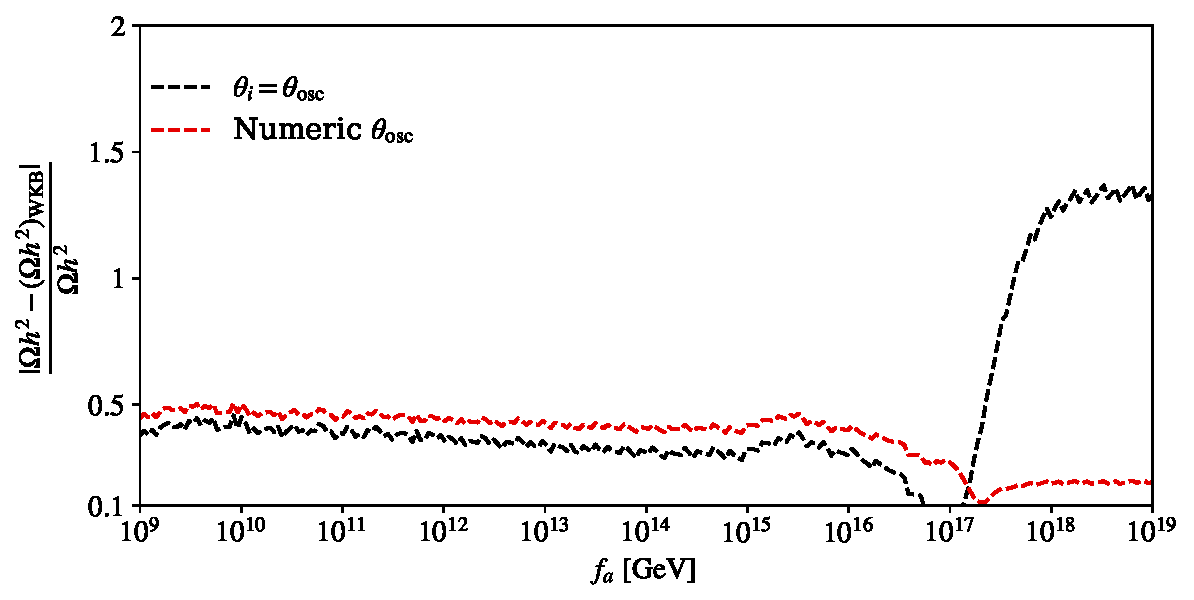
\includegraphics[width=1\textwidth]{figs/RD_WKB_diff.pdf}
		\caption{}
		\label{fig:RD_WKB_diff}
	\end{subfigure}
	\begin{subfigure}[]{0.5\textwidth}
		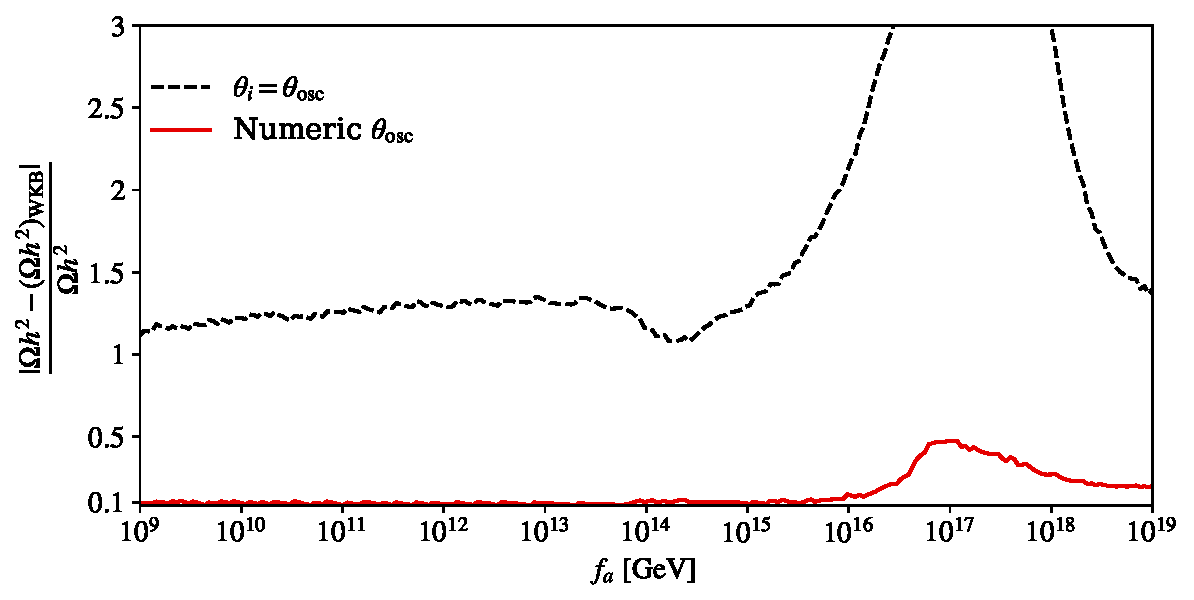
\includegraphics[width=1\textwidth]{figs/NSC_WKB_diff.pdf}
		\caption{}
		\label{fig:NSC_WKB_diff}
	\end{subfigure}
	\begin{center}
		\begin{subfigure}[]{.5\textwidth}
		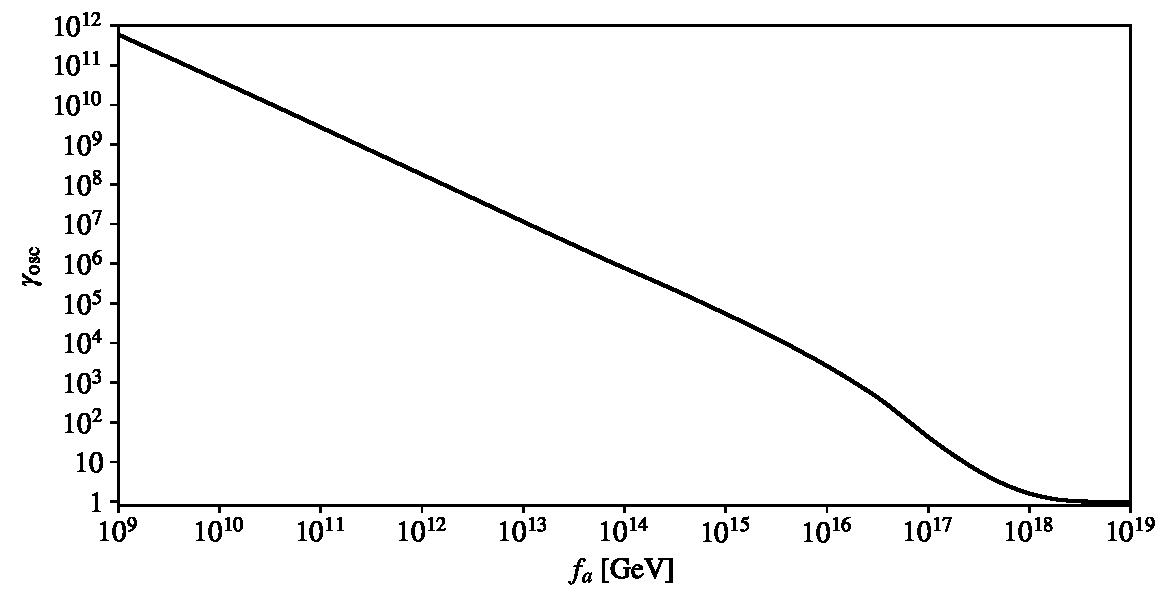
\includegraphics[width=1\textwidth]{figs/gamma_osc.pdf}
		\caption{}
		\label{fig:gamma_osc}
	\end{subfigure}
	\end{center}
\caption{...}
\label{fig:WKB_diff}
\end{figure}
%

\subsubsection{Adiabatic invariant and the anharmonic factor}\label{sec:an_fac}
%
In oscillatory systems with varying period, the energy is not conserved, and it is usually useful to define an ``adiabatic invariant", which is an approximate constant of motion.

\paragraph{Definition of the adiabatic invariant}
%
Given a system with Hamiltonian $\mathcal{H}(\theta,p;t)$, the equations of motion are 
%
\begin{equation}
	\dot p = - \dfrac{\partial \mathcal{H}}{\partial \theta} \;, \;\; 
	\dot \theta =  \dfrac{\partial \mathcal{H}}{\partial p} \;.
	\label{eq:hamiltonian_eoms}
\end{equation}

Moreover, we note that
%
\begin{equation}
	d \Ham = \dot \theta \ d p - \dot p \ d \theta + \dfrac{\partial \Ham}{\partial t} \ d t \;.  
	\label{eq:total_dH}
\end{equation}


If this system exhibits closed orbits (\eg if it oscillates), we define 
%
\begin{equation}
	J \equiv C \ \oint p \ d \theta \;,
	\label{eq:adiabatic_inv_def}
\end{equation}
%
where the integral is over a closed path (\eg a period, $T$), and $C$ indicates that $J$ can always be rescaled with a constant. This quantity is the adiabatic invariant of the system, if the Hamiltonian varies slowly during a cycle. That is,
%
\[
\dfrac{d J}{d t} = C \ \oint \lrBigb{\dot p \ d \theta + p \ d \dot \theta} = C \ \dint_{t}^{t+T}  \dfrac{\partial \Ham}{\partial t^\prime} \ d t^\prime \approx T \ \dfrac{\partial \Ham(t^{\prime})}{\partial t^{\prime}}\Big|_{t^{\prime}=t} \approx 0 
\;. 
\]
%




\paragraph{Application to the axion}
%
The Hamiltonian that results in the EOM of \eqs{eq:eom} is
%
\begin{equation}
	\Ham = \dfrac{1}{2} \dfrac{p^2}{\fa^2 \ R^3} + V(\theta) \ R^3\;,
	\label{eq:axion_H}
\end{equation}
%
with 
%
\begin{eqnarray}
	& p = \fa^2 \ R^3 \ \dot \theta \\
	\label{eq:momentum}
	& V(\theta) = \maT^2 \fa^2 (1-\cos \theta) \;.
	\label{eq:potential}
\end{eqnarray}

Notice that the Hamiltonian varies slowly if $\dot \maT/\maT \ll \maT$ and $H \ll \maT$, which are the adiabatic conditions.  When these conditions are met, the adiabatic invariant for this system becomes
%
\begin{equation}
	J = \dfrac{\oint p \ d \theta}{\pi \fa^2} = \dfrac{1}{\pi \fa^2} \oint \sqrt{ 2\lrb{ \Ham(\theta) - V(\theta) \ R^3} \ \fa^2 R^3 \ }  \ d \theta  =
	 \dfrac{2}{\pi \fa^2} \int_{-\thetamax}^{\thetamax} \sqrt{ 2\lrb{ \Ham(\thetamax) - V(\theta) \ R^3} \ \fa^2 R^3 \ } d \theta \;,
	 \label{eq:J_axion_definition}
\end{equation}
%
where we note that $\thetamax$ denotes the maximum of $\theta$ -- the peak of the oscillation, which corresponds to $p=0$. That is, $\Ham(\thetamax) = V(\thetamax) \ R^3$. Therefore, the adiabatic invariant, takes the form 

\begin{eqnarray}
	J=&  \dfrac{2 \sqrt{2} }{\pi \fa}  \int_{- \thetamax} ^{\thetamax}  \sqrt{ V(\theta_{\rm max}) - V(\theta) } R^{3} d \theta = 
	\dfrac{2 \sqrt{2} }{\pi} \ \maT \, R^3 \ \dint_{- \thetamax}^{\thetamax} \sqrt{\cos \theta - \cos \thetamax} \ d \theta  
	\;,
	\label{eq:J_axion_derivation}
\end{eqnarray}
%
where, for the last equality. we have used the adiabatic conditions, \ie negligible change of $\maT$ and $R$ during one period. Usually, the adiabatic invariant is written as~\cite{Lyth:1991ub,Bae:2008ue} 
%
\begin{equation}
	J = R^3 \ \maT \ \thetamax^2  \, f(\thetamax)  \;,
	\label{eq:J_axion_final_form}
\end{equation}
%
where 
\begin{equation}
	f(\thetamax) =\dfrac{ 2 \sqrt{2}}{\pi \thetamax^2 } \dint_{- \thetamax}^{\thetamax} d \theta \sqrt{ \cos \theta - \cos \thetamax } \;,
	\label{eq:anharmonic_f}
\end{equation}
%
is called the anharmonic factor, with $ 0.5 \lesssim f(\thetamax) \leq 1$ (see \Figs{fig:anharmonic_factor}).


\begin{figure}[t]
	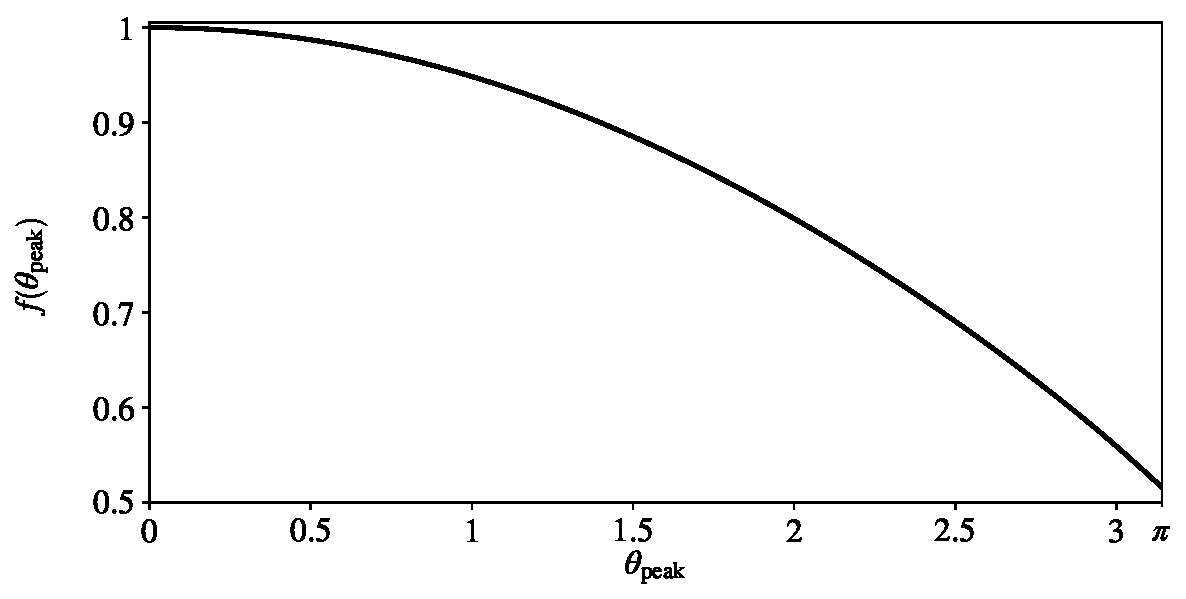
\includegraphics[width=1\textwidth]{figs/anharmonic_factor.pdf}
	\caption{The anharmonic factor for $0 \leq \thetamax < \pi $.}
	\label{fig:anharmonic_factor}
\end{figure}



\paragraph{The role of the adiabatic invariant in the axion relic energy density}
%
The adiabatic invariant allows us to calculate the maximum value of the angle $\theta$ at late times from its corresponding value at some point after the adiabatic conditions where met. It allows us to calculate the energy density of the axions field for $\theta \gtrsim 1$ since we have taken into account the exact potential.

In order to do this, we can numerically integrate \eqs{eq:eom}, and identify the maxima of $\theta$. Once the adiabatic conditions are fulfilled, we can stop the integration at a peak, $\thetamax_{,*}$ -- which corresponds to $T=T_{*}$ and $R=R_{*}$. Then, the value of the maximum angle today ($\thetamax_{,0} \ll 1$) is related to $\thetamax_{,*}$ via
%
\begin{eqnarray}
	\thetamax_{,0}^2 &=  \lrb{\dfrac{R_*}{R_0}}^3 \ \dfrac{\maT_{,*}}{\ma} \ f(\thetamax_{,*}) \ \thetamax_{,*}^2  =
	\gamma^{-1} \ \dfrac{s_0}{s_*} \ \dfrac{\maT_{,*}}{\ma} \ f(\thetamax_{,*}) \ \thetamax_{,*}^2 
	\; .
	\label{eq:theta_relation}
\end{eqnarray}
%
Using this, and since we evaluate the energy density at the maximum of $\theta$ (\ie $\dot \theta = 0$), we can determine the energy density of axions today from \eqs{eq:rho_a_def}. That is,
%
\begin{equation}
	\rho_{a,0} = \gamma^{-1} \ \dfrac{s_0}{s_*} \ \ma \ \maT_{,*} \ \dfrac{1}{2} \ \fa^2 \ \thetamax_{,*}^2 \;  \ f(\thetamax_{,*}) \;.
	\label{eq:rho_axion_exact}
\end{equation}
%
Notice that this is form of $\rho_{a,0}$  is similar to the the WKB result~(\ref{eq:rho_a_approx}) at $\tosc \to t_*$, multiplied by the anharmonic factor $f(\thetamax_{,*})$. That is, if the axion starts to evolve adiabatically close to $t=\tosc$, and $\thetaosc \ll 1$, the WKB approximation is valid.






\section{How to start using \mimes}\label{sec:start}
\setcounter{equation}{0}

The library can downloaded from \href{https://github.com/dkaramit/MiMeS}{github.com/dkaramit/MiMeS}. Once download is complete, we can go inside the \mimes directory, and run {\tt bash configure.sh} and  {\tt make}.  The {\tt bash} script {\tt configure.sh}, downloads parts of {\tt NaBBODES} and {\tt SimpleSplines}~\footnote{\href{https://github.com/dkaramit/NaBBODES}{\tt NaBBODES} is header-only library for ODE integration, and \href{https://github.com/dkaramit/SimpleSplines}{\tt SimpleSplines} is header-only library for spline interpolation.}, writes some files, and  makes some directories, needed \mimes. The {\tt makefile} is responsible for compiling some examples and checks, as well as the shared libraries that we need, for the \PY interface.  If everything runs successfully, there should be two new directories {\tt exec} and {\tt lib}. Inside {\tt exec}, there are several executables that we can run, in order to ensure that the code runs (\eg no segmentation fault occurs). For example, {\tt exec/AxionSolve\_check.run}, should print the values of the parameters $\thetai$ and $\fa$, the oscillation temperature and the corresponding value of $\theta$, the evolution of the axion (\eg temperature, $\theta$, $\rho_{a}$, etc.), and the values of various quantities on the peaks of the oscillation.  In the directory {\tt lib}, there are several shared libraries, that the \PY interface needs.

\paragraph{First steps} There are several examples in \CPP ({\tt Examples/Cpp}) and \PY ({\tt Examples/Python}), as well as \JUPY  notebooks ({Examples/JupyterNotebooks} and {\tt Examples/scan}), that show in detail how \mimes can be used.

\paragraph{Using \mimes in \CPP} \DK{Describe the {\tt mimes::Axion} class}.

\paragraph{Using \mimes in \PY} \DK{Describe the {\tt Axion} class in {\tt interfacePy.Axion} module}.


\section{Assumptions and user input}\label{sec:assumptions}
\setcounter{equation}{0}

\mimes makes only a few, fairly general assumptions. First of all, it is assumed that the axion energy density is always subdominant compared to radiation or any other component of the Universe, and that decays and annihilations of particles have a negligible effect on the axion energy density. Moreover, the initial condition are always assumed to be $\thetai = const$ (\ie $\dot \theta|_{t=\ti}=0$).

\DK{since you have described the classes, you can now talk about {\tt ratio\_ini} and the others!}




\newpage
%%%%%%%%%%%%%%%%%%%%%%%%%%%%%%%
 \bibliography{refs}{}
 \bibliographystyle{JHEP}                        

\end{document}
